\graphicspath{{chapters/gradient_descent/}}
\chapter{Efficient Algorithms for the CCA Family: Unconstrained Losses with Unbiased Gradients}\label{chap:gradient_descent}
\epigraph{It seems easier to train a bi-directional LSTM with attention than to compute the SVD of a large matrix.\cite{gemp}}{Chris Ré}
\minitoc
% chktex-file 44
% chktex-file 3
\section*{Preface}
The content of this chapter is based on a series of papers~\citep{chapman2022generalized, chapman2023efficient} as well as a NeurIPS workshop paper~\citep{chapman2023neurips}.
I am grateful to my co-authors Lennie Wells and Ana Lawry Aguila for their contributions to this work.
In particular, Lennie's mathematical expertise improved the theoretical grounding of the idea greatly and Ana's access to the UK Biobank dataset enabled the application of our methods to a real-world biomedical dataset.
In this thesis I include much of the work from these papers, but I exclude many of Lennie's extensive proofs where I can make no claim to have contributed beyond proofreading.
It was a joy to bring this work to fruition and I am proud of the results we achieved.

\section{Introduction}

\section{Background: A unified approach to the CCA family}\label{sec:background-unified}

Suppose we have a sequence of vector-valued random variables $X^{(i)} \in \R^{D\sps{i}}$ for $i \in \{1, \dots, I \}$\footnote{Yes, there are I (eye) views}.
We want to learn meaningful $K$-dimensional representations
\begin{equation}\label{eq:general-form-of-representations}
    Z\sps{i} = f\sps{i}( X\sps{i}; \theta\sps{i}).
\end{equation}
For convenience, define $D = \sum_{i=1}^I D\sps{i}$ and $\theta = \left(\theta\sps{i}\right)_{i=1}^I$.
%Without loss of generality take $D\sps{1} \geq D\sps{2} \geq \cdots \geq D\sps{I}$.
We will consistently use the superscripts $i,j \in [I]$ for views
%subscripts $d \in [D\sps{i}]$ for dimensions of input variables;
and subscripts $l,k \in [K]$ for dimensions of representations - i.e. to subscript dimensions of $Z\sps{i}, f\sps{i}$.
Later on we will introduce total number of samples $N$ and mini-batch size $M$.
%so we will subscript samples with $n,m$ respectively.
% don't know if actually ended up using this, so can comment out if not!

\subsection{Background: GEPs in linear algebra}
A Generalized Eigenvalue Problem (GEP) is defined by two symmetric matrices $A,B\in \mathbb{R}^{D\times D}$ \citep{stewart_matrix_1990}\footnote{more generally, $A,B$ can be Hermitian, but we are only interested in the real case}. They are usually characterized by the set of solutions to the equation:
\begin{align}\label{eq:igep}
Au=\lambda Bu
\end{align}
with $\lambda \in \R, u \in \R^D$, called (generalized) eigenvalue and (generalized) eigenvector respectively. We shall only consider the case where $B$ is positive definite to avoid degeneracy.
Then the GEP becomes equivalent to an eigen-decomposition of the symmetric matrix $B^\mhalf A B^\mhalf$. This is key to the proof of our new characterization.
In addition, one can find a basis of eigenvectors spanning $\R^D$.
%the eigenvectors are not always unique, but the eigenvalues $\lambda_1 \geq \dots \geq \lambda_d$ are.
We define a \textit{top-$K$ subspace} to be one spanned by some set of eigenvectors {$u_1,\dots,u_K$} with the top-$K$ associated eigenvalues $\lambda_1 \geq \dots \geq \lambda_K$.
We say a matrix $U \in \R^{D \times K}$ \textit{defines} a top-$K$ subspace if its columns span one.
%hoping this finesses non-uniqueness for main text.
% GEPs have a rich geometric structure, and lead to many alternative characterizations, such as the following constrained characterization from \citep{stewart_matrix_1990}.

% \begin{restatable}[Constrained objective for GEPs]{proposition}{GEPconstrained}
% \label{prop:GEP-constrained}
%     The top-$K$ subspace of the GEP $(A,B)$ can be characterized by the following maximization \begin{equation}\label{eq:gep-constrained-subspace-formulation}
%         \max_{U \in \R^{d\times k}} \tr(U^{\top} A U) \quad \text{ subject to: }  U^{\top} B U = I_K.
%         \end{equation}
%     Moreover, the maximal value of this objective is $\sum_{k=1}^K \lambda_k$.
% \end{restatable}


\subsection{The CCA Family}\label{sec:CCA-family}
The classical notion CCA \citep{hotelling1992relations} considers two views, $I=2$, and constrains the representations to be linear transformations
\begin{equation}\label{eq:cca-linear-function-def}
    Z\sps{i}_k = \langle u_k\sps{i} , X\sps{i} \rangle.
\end{equation}

The objective is to find the \textit{weights} or \textit{canonical directions} $u_k\sps{i}$ which maximize the \textit{canonical correlations} $\rho_k = \Corr(Z\sps{1}_k, Z\sps{2}_k)$
sequentially, subject to orthogonality with the previous pairs of the transformed variables.
It is well known that CCA is equivalent to a singular value decomposition (SVD) of the matrix $\Var(X\sps{1})^\mhalf \Cov(X\sps{1}, X\sps{2}) \Var(X\sps{2})^\mhalf$.
It is slightly less well known \citep{borga_learning_1998} that this is equivalent to a GEP where:
\begin{equation}\label{eq:cca-GEV}\small
	A = \begin{pmatrix} 0 &\Cov(X\sps{1}, X\sps{2}) \\ \Cov(X\sps{2}, X\sps{1}) & 0 \end{pmatrix}, \quad
	B = \begin{pmatrix}\Var(X\sps{1}) & 0 \\ 0 & \Var(X\sps{2}) \end{pmatrix}, \quad
	u =\begin{pmatrix}	u\sps{1} \\ u\sps{2} \end{pmatrix}.
\end{equation}

CCA therefore has notions of uniqueness similar to those for SVD or GEPs: the weights are not in general unique, but the canonical correlations $1 \geq \rho_1 \geq \rho_2 \geq \dots \geq 0$ are unique \citep{mills1988calculation}. Therefore, we can write:
%\footnote{Slightly abusing notation: $\CCA_K$ is a function of the joint distribution $\mathcal{L}_{X\sps{1}, \sps{2}}$ not of the random vectors themselves}:
\begin{align}\label{eq:cca-vector-of-correlations-def}\small
    \CCA_K(X^{(1)},X^{(2)}) \defeq (\rho_k)_{k=1}^K
    %= \sigma_{1, \dots, K} \left(\Var(X\sps{1})^\mhalf \Cov(X\sps{1}, X\sps{2}) \Var(X\sps{2})^\mhalf\right).
\end{align}


\textbf{Sample CCA:} in practice we do not have access to the population distribution but to a finite number of samples; the classical estimator is defined by replacing the population covariances in \cref{eq:cca-GEV} with sample covariances.
Unfortunately, this estimator breaks down when $N \leq \max(D\sps{1}, D\sps{2})$; giving arbitrary correlations of 1 and meaningless directions\footnote{WLOG take $D\sps{1} \geq \max(N, D\sps{2})$. Then for any given observations $\X\sps{1} \in \R^{N \times K}, \Z\sps{2}_k \in \R^N$ there exists some $u_k\sps{1}$ such that $\X\spsT{1} u_k\sps{1} = \Z\sps{2}_k$ - provided the observations of $\X\sps{1}$ are not linearly dependent - which is e.g. true with probability 1 when the observations are drawn from a continuous probability distribution.}.

\textbf{Ridge-regularized CCA:} the most straightforward way to prevent this overfitting is to add a ridge regularizer \citep{vinod1976canonical}.
Taking maximal ridge regularization recovers \textbf{Partial Least Squares PLS} \citep{mihalik_canonical_2022}, a widely used technique for multi-view learning.
Even these simple modifications to CCA can be very effective at preventing overfitting in high dimensions \citep{mihalik_canonical_2022}.

\textbf{Multi-view CCA (MCCA):} extends two-view CCA to deal with three or more views of data. Unfortunately, many of the different equivalent formulations of two-view CCA are no longer equivalent in the multi-view setting, so there are many different extensions to choose from; see \cref{sec:related-work}. Of most interest to us is the formulation of \cite{nielsen2002multiset, wong2021deep} that extends the GEP formulation of \cref{eq:cca-GEV}, which we next make precise and will simply refer to as MCCA from now.
% Applying the general formulation of \cref{eq:def-general-constrained-objective} to the linear \cref{eq:cca-linear-function-def} multi-view setting we derive a version Multiset CCA (MCCA) \cite{wong2021deep, nielsen2002multiset}.

\textbf{Unified GEP formulation:}
this GEP formulation of MCCA can be presented in a unified framework generalizing CCA and ridge-regularized extensions. Indeed, we now take $A,B_\alpha \in \R^{D \times D}$ to be block matrices $A = (A\sps{ij})_{i,j=1}^I, B_\alpha = (B_\alpha\sps{ij})_{i,j=1}^I$ where the diagonal blocks of $A$ are zero, the off-diagonal blocks of $B_\alpha$ are zero, and the remaining blocks are defined by:
\begin{align}\label{eq:gep-most-general-formulation}%\small
    A^{(ij)} &= \Cov(X\sps{i}, X\sps{j}) \text{ for } i \neq j, \quad % \text{ for } i,j \in [I], ; \:\:
    B_\alpha^{(ii)} = \alpha_i I_{D\sps{i}} + (1-\alpha_i) \Var(X\sps{i})  %\text{ for } i \in [I]
\end{align}
Where $\alpha \in [0,1]^I$ is a vector of ridge penalty parameters: taking $\alpha_i = 0 \: \forall i$ recovers CCA and $\alpha = 1 \: \forall i$ recovers PLS.
We may omit the subscript $\alpha$ when $\alpha=0$ and we recover the `pure CCA' setting; in this case, following \cref{eq:cca-vector-of-correlations-def} we can define $\MCCA_K(X\sps{1},\dots,X\sps{I})$ to be the vector of the top-$K$ generalized eigenvalues.


\textbf{Deep CCA:} was originally introduced in \cite{andrew2013deep}; this was extended to an GEP-based formulation of \textbf{Deep Multi-view CCA} (DMCCA) in \cite{somandepalli2019multimodal}. This can be defined using our $\MCCA$ notation as maximizing
\begin{align}\label{eq:DMCCA-def}
    \norm{\MCCA_K\left(Z\sps{1}, ... Z\sps{I}\right)}_2
    %=\norm{V(\theta)^\mhalf C(\theta) V(\theta)^\mhalf}_F
\end{align}
over parameters $\theta$ of neural networks defining the representations $Z\sps{i}=f\sps{i}(X\sps{i};\theta\sps{i})$ for $i\in[I]$.
% which of course generalizes Andrew version
% $\norm{\CCA_K\left(Z\sps{1}, Z\sps{2}\right)}_2 =
%     \norm{\Var(Z\sps{1})^\mhalf \Cov(Z\sps{1}, Z\sps{2}) \Var(Z\sps{2})^\mhalf}_F$

\section{Novel Objectives and Algorithms}\label{sec:contributions}
\subsection{Unconstrained objective for GEPs}\label{sec:gep-ey-formulation}
First, we present proposition \ref{prop:EY-charac}, a formulation of the top-$K$ subspace of GEP problems, which follows by applying the Eckhart--Young--Minsky inequality \citep{stewart_matrix_1990} to the eigen-decomposition of $B^\mhalf A B^\mhalf$. However, making this rigorous requires some technical care which we defer to the proof in supplement \ref{supp:proofs}.

\begin{restatable}[Eckhart--Young inspired objective for GEPs]{proposition}{EYcharac}
\label{prop:EY-charac}
    The top-$K$ subspace of the GEP $(A,B)$ can be characterized by minimizing the following objective over $U \in \R^{D \times K}$:
    \begin{align}\label{eq:EY-charac}
        \LEYGEP(U) \defeq \tr \left( - 2\,U^T A U + \left(U^T B U\right) \left(U^T B U\right) \right)
    \end{align}
    Moreover, the minimum value is precisely $- \sum_{k=1}^K \lambda_k^2$, where $(\lambda_k)$ are the generalized eigenvalues.
\end{restatable}

This objective also has appealing geometrical properties.
It is closely related to a wide class of unconstrained objectives for PCA and matrix completion which have no spurious local optima \citep{ge_no_2017}, i.e. all local optima are in fact global optima.
This implies that certain local search algorithms, such as stochastic gradient descent, should indeed converge to a global optimum.

\begin{restatable}{proposition}{NoSpuriousLocalMinima}[No spurious local minima]\label{prop:no-spurious}
    The objective $\LEYGEP$ has no spurious local minima.
    That is, any matrix $\bar{U}$ that is a local minimum of $\LEYGEP$ must in fact be a global minimum.
    %of the form described in \cref{prop:EY-charac}
\end{restatable}

It is also possible to make this argument quantitative by proving a version of the strict saddle property from \cite{ge_no_2017,ge2015escaping}; we state an informal version here and give full details in \cref{supp:tractable-optimization}.

\begin{corollary}[Informal: Polynomial-time Optimization]
    Under certain conditions on the eigenvalues and generalized eigenvalues of $(A,B)$, one can make quantitative the claim that:
    any $U_K \in \R^{D \times K}$ is either close to a global optimum, has a large gradient $\nabla \LEYGEP$, or has Hessian $\nabla^2 \LEYGEP$ with a large negative eigenvalue.

    Therefore, for appropriate step-size sequences, certain local search algorithms, such as sufficiently noisy SGD, will converge in polynomial time with high probability.
    % still need to sort out - polynomial in what exactly!
\end{corollary}

\subsection{Corresponding Objectives for the CCA family}
For the case of linear CCA we have $U^T A U = \sum_{i \neq j} \Cov(Z\sps{i}, Z\sps{j}), U^T B U = \sum_{i} \Var(Z\sps{i})$.
To help us extend this to the general case of nonlinear transformations, \cref{eq:general-form-of-representations}, we define the analogous matrices of total between-view covariance and total within-view variance
\begin{align}\label{eq:def-C-V-matrices}
    \vphantom{\bigl(\bigr)} % increase vertical space
    C(\theta) = \sum_{i \neq j} \Cov(Z\sps{i}, Z\sps{j}), \quad
    V(\theta) = \sum_{i} \Var(Z\sps{i})
\end{align}
In the case of linear transformations, \cref{eq:cca-linear-function-def}, it makes sense to add a ridge penalty so we can define
\begin{align}\label{eq:v-alpha-ridge-definition}
    V_\alpha(\theta) = \sum_i \alpha_i {U\spsT{i}} U\sps{i} +  (1 - \alpha_i) \Var(Z\sps{i})
\end{align}
This immediately leads to following unconstrained objective for the CCA-family of problems.
\begin{definition}[Family of EY Objectives]
    Learn representations $Z\sps{i} = f\sps{i}( X\sps{i}; \theta\sps{i})$ minimizing
    \begin{align}\label{eq:EY-loss-def-C-V}
        \LEY(\theta) = - 2 \tr C(\theta) + \norm{V_\alpha(\theta)}_F^2
    \end{align}
\end{definition}

\textbf{Unbiased estimates:}
since empirical covariance matrices are unbiased, we can construct unbiased estimates to $C, V$ from a batch of transformed variables $\Z$.
\begin{align}\label{eq:def-C-V-matrices-empirical}
    \hat{C}(\theta)[\Z] = \sum_{i \neq j} \empCov(\Z\sps{i}, \Z\sps{j}), \quad
    \hat{V}(\theta)[\Z] = \sum_{i} \empVar(\Z\sps{i})
\end{align}
In the linear case we can construct $\hat{V}_\alpha(\theta)[\Z]$ analogously by plugging sample covariances into \cref{eq:v-alpha-ridge-definition}.
Then if $\Z, \Z'$ are two independent batches of transformed variables, the batch loss
\begin{align}\label{eq:empirical-EY-loss-estimate-def}
    \empLEY[\Z, \Z'] \defeq - 2 \tr \hat{C}[\Z] + \langle \hat{V}_\alpha[\Z], \hat{V}_\alpha[\Z'] \rangle_F
\end{align}
gives an unbiased estimate of $\LEY(\theta)$.%\footnote{Where again $\alpha > 0$ only makes sense in the linear case, and otherwise we may omit the $\alpha$s}
This loss is a differentiable function of $\Z, \Z'$ and so also of $\theta$.

\textbf{Simple algorithms:}
We first define a very general algorithm using these estimates in Algorithm \ref{alg:general}.
In the next section we apply this algorithm to multi-view stochastic CCA and PLS, and Deep CCA.

\begin{algorithm}
   \caption{GEP-EY: General algorithm for learning correlated representations}
   \label{alg:general}
\begin{algorithmic}
   \STATE {\bfseries Input:} data stream of mini-batches $(\X(b))_{b=1}^\infty$ where each consists of $M$ samples from the original dataset. Learning rate $(\eta_t)_t$. Number of time steps $T$. Class of functions $f(\cdot; \theta)$ whose outputs are differentiable with respect to $\theta$.
   \STATE {\bfseries Initialize:} $\hat{\theta}$ with suitably random entries
   \FOR{$t=1$ {\bfseries to} $T$}
       \STATE Obtain two independent mini-batches \( \X(b), \X(b') \) by sampling \( b, b' \) independently
       \STATE Compute batches of transformed variables $\Z(b) = f(\X(b); \theta), \Z(b') = f(\X(b'); \theta)$
       %\STATE Construct unbiased estimates $C(\theta)[\Z], \hat{V}(\theta)[\Z], \hat{V}(\theta)[\Z']$ \COMMENT{As defined in \cref{eq:def-C-V-matrices-empirical}}
       \STATE Estimate loss $\empLEY(\theta)$ using \cref{eq:empirical-EY-loss-estimate-def}
       \STATE Obtain gradients by back-propagation and step with your favourite optimizer.
   \ENDFOR
\end{algorithmic}
\end{algorithm}

\subsection{Applications to (multi-view) stochastic CCA and PLS, and Deep CCA}
\begin{lemma}[Objective recovers GEP formulation of linear (multi-view) CCA]
    When the $f\sps{i}$ are linear, as in \cref{eq:cca-linear-function-def}, the population loss from \cref{eq:EY-loss-def-C-V} recovers MCCA as defined in \cref{sec:CCA-family}. %Moreover, the minimal loss value is precisely $-\norm{\MCCA_K(X)}$
\end{lemma}
\begin{proof}
    By construction, for linear MCCA we have $C = U^T A U,\, V_\alpha=U^T B_\alpha U$, where $(A, B_\alpha)$ define the GEP for MCCA introduced in \cref{eq:gep-most-general-formulation}.
    So $\LEY(U) = \LEYGEP(U)$ and by \cref{prop:EY-charac} the optimal set of weights define a top-$K$ subspace of the GEP, and so is a MCCA solution.
    %; by definition, $\MCCA_K$ is the vector of top-$K$ generalised eigenvalues, so the optimal value is as claimed.
\end{proof}

Moreover, by following through the chain of back-propagation, we obtain gradient estimates in $\mathcal{O}(MKD)$ time.
Indeed, we can obtain gradients for the transformed variables in $\mathcal{O}(M K^2)$ time so the dominant cost is then updating $U$; we flesh this out with full details in \cref{supp:fast-updates}.

\begin{restatable}{lemma}{recoverDeepCCA}[Objective recovers Deep Multi-view CCA]\label{lem:recover-DeepCCA}
    Assume that there is a final linear layer in each neural network $f\sps{i}$.
    Then at any local optimum, $\hat{\theta}$, of the population problem, we have
    \begin{align*}
        \LEY(\hat{\theta}) = - \norm{\MCCA_K(\hat{Z})}_2^2
    \end{align*}
    where $\hat{Z} = f_{\hat{\theta}}(X)$.
    Therefore, $\hat{\theta}$ is also a local optimum of objectives from \cite{andrew2013deep, somandepalli2019multimodal} as defined in \cref{eq:DMCCA-def}.
\end{restatable}
\begin{proof}[Proof sketch: see \cref{supp:EY-recover-Deep-CCA} for full details.]
    Consider treating the penultimate-layer representations as fixed, and optimising over the weights in the final layer. This is precisely equivalent to optimising the Eckhart-Young loss for linear CCA where the input variables are the penultimate-layer representations. So by \cref{prop:no-spurious}, a local optimum is also a global optimum, and by \cref{prop:EY-charac} the optimal value is the negative sum of squared generalised eigenvalues.
\end{proof}

\subsection{Application to SSL}
We can directly apply Algorithm \ref{alg:general} to SSL.
If we wish to have the same neural network transforming each view, we can simply tie the weights $\theta\sps{1} = \theta\sps{2}$.
When the paired data are generated from applying independent, identically distributed (i.i.d.) augmentations to the same original datum, it is intuitive that tying the weights is a sensible procedure, and perhaps acts as a regulariser.
We make certain notions of this intuition precise for CCA and Deep CCA in \cref{supp:further-cca}.

To provide context for this proposal, we also explored in detail how VICReg and Barlow twins are related to CCA.
For now we focus on VICReg, whose loss can be written as
\begin{small}\begin{align*}
    \mathcal{L}_\text{VR}(Z\sps{1}, Z\sps{2})
    &= \gamma \mathbb{E} \norm{Z^{(1)} - Z^{(2)}}^2 + \sum_{i \in \{1,2\}} \bigg[\alpha \sum_{k=1}^K \left(1 \shortminus \sqrt{\Var(Z\sps{i}_i)}\right)_+ + \beta \sum_{\substack{k,l=1 \\ k \neq l}}^K \Cov(Z\sps{i}_k,Z\sps{i}_l)^2 \bigg]
\end{align*}\end{small}%
where $\alpha, \beta, \gamma > 0$ are tuning parameters and, as in the framework of \cref{sec:background-unified}, the $Z\sps{1}, Z\sps{2}$ are $K$-dimensional representations, parameterised by neural networks in \cref{eq:general-form-of-representations}.
Our main conclusions regarding optima of the population loss are:
\begin{itemize}
    \item Consider the linear setting with untied weights. Then global optimisers of the VICReg loss define CCA subspaces, but may not be of full rank.
    \item Consider the linear setting with tied weights and additionally assume that the data are generated by i.i.d. augmentations. Then the same conclusion holds.
    \item In either of these settings, the optimal VICReg loss is a component-wise decreasing function of $\CCA_K(X\sps{1}, X\sps{2})$ the vector of population canonical correlations.
    \item VICReg can therefore be interpreted as a formulation of Deep CCA, but one that will not in general recover full rank representations.
\end{itemize}

% We believe versions of each of these conclusions also hold for Barlow twins, but can only prove a subset of the results at present.%, see \cref{supp:ssl-theory} for further discussion.
We give full mathematical details and further discussion in \cref{supp:ssl-theory}.
The analysis for Barlow twins is more difficult, but we present a combination of mathematical and empirical arguments which suggest all the same conclusions hold, again see \cref{supp:ssl-theory}.

\section{Related Work}\label{sec:related-work}

\textbf{Stochastic PLS and CCA:}
To the best of our knowledge, the state-of-the-art in Stochastic PLS and CCA are the subspace Generalized Hebbian Algorithm (\textbf{SGHA}) of \cite{chen2019constrained} and \textbf{$\gamma$-EigenGame} from \cite{gemp20,gemp2021}. Specifically, SGHA utilizes a Lagrange multiplier heuristic along with saddle-point analysis, albeit with limited convergence guarantees. EigenGame focuses on top-k subspace learning but introduces an adaptive whitening matrix in the stochastic setting with an additional hyperparameter. Both methods set the benchmarks we aim to compare against in the subsequent experimental section. Like our method, both can tackle other symmetric Generalized Eigenvalue Problems in principle.

\textbf{DCCA and Deep Multiview CCA:}
The deep canonical correlation analysis (DCCA) landscape comprises three principal approaches with inherent limitations. The first, known as the full-batch approach, uses analytic gradient derivations based on the full sample covariance matrix \citep{andrew2013deep}.
% Lennie: could work in $\norm{\Var(Z\sps{1})^\mhalf \Cov(Z\sps{1}, Z\sps{2}) \Var(Z\sps{2})^\mhalf}_F$ here - what do you think James?
The second involves applying the full batch objective to large mini-batches, an approach referred to as \textbf{DCCA-STOL} \citep{wang2015unsupervised}. However, this approach gives biased gradients and therefore requires batch sizes much larger than the representation size in practice. This is the approach taken by both \textbf{DMCCA} \citep{somandepalli2019multimodal} and \textbf{DGCCA} \citep{benton2017deep} . The final set of approaches use an adaptive whitening matrix \citep{wang2015stochastic, chang2018scalable} to mitigate the bias of the Deep CCA objective. However, the authors of \textbf{DCCA-NOI} highlight that the associated time constant complicates analysis and requires extensive tuning. These limitations make existing DCCA methods less practical and resource-efficient.


\textbf{Self-Supervised Learning:}
\textbf{Barlow Twins} and \textbf{VICReg} have come to be known as part of the canonical correlation family of algorithms \citep{balestriero2023cookbook}. Barlow Twins employs a redundancy reduction objective to make the representations of two augmented views both similar and decorrelated \citep{zbontar2021barlow}. Similarly, VICReg uses variance-invariance-covariance regularization, which draws upon canonical correlation principles, to achieve robust performance in diverse tasks \citep{bardes2021vicreg}. These methods serve as vital baselines for our experiments, owing to their foundational use of canonical correlation ideas.

\section{Experiments}\label{Experiments}

% Stochastic CCA Section
\subsection{Stochastic CCA}
First, we compare our proposed method, CCA-EY, to the baselines of $\gamma$-EigenGame and SGHA.
Our experimental setup is almost identical to that of \cite{meng2021online, gemp2022generalized}; unlike \cite{gemp2022generalized} we do not simplify the problem by first performing PCA on the data before applying the CCA methods, which explains the decrease in performance of $\gamma$-EigenGame compared to their original work.
All models are trained for a single epoch with varying mini-batch sizes ranging from 5 to 100. We use Proportion of Correlation Captured (PCC) as our evaluation metric, defined as \( \text{PCC} = (\sum_{i=k}^K \rho_k)/ ({\sum_{k=1}^K \rho_k^*}) \) where $\rho_k$ are the full batch correlations of the learnt representations, and $\rho_k^*$ are the canonical correlations computed numerically from the full batch covariance matrices.

% In this section, we assess the performance of our proposed method, CCA-EY, against baseline techniques $\gamma$-EigenGame and SGHA. We draw upon the experimental setups detailed in \cite{meng2021online, gemp2022generalized}, zeroing in on the MediaMill dataset to evaluate top-5 canonical correlations. Our models are trained for a single epoch with varying mini-batch sizes ranging from 5 to 100. We utilize the Proportion of Correlation Captured (PCC), defined as \( \text{PCC} = \frac{\sum_{i=1}^k \rho_i}{\sum_{i=1}^k \rho_i^*} \), as our evaluation metric.

\textbf{Observations:}
Figure \ref{fig:scca_mediamill} compares the algorithms on the MediaMill dataset. \cref{fig:corr_mediamill} shows that CCA-EY consistently outperforms both $\gamma$-EigenGame and SGHA in terms of PCC across all evaluated mini-batch sizes.
\cref{fig:lr_mediamill} examines the learning curves for batch sizes 5 and 100 in more detail; CCA-EY appears to learn more slowly than SGHA at the start of the epoch, but clearly outperforms SGHA as the number of samples seen increases. $\gamma$-EigenGame significantly underperforms SGHA and CCA-EY, particularly for small batch sizes.

\textbf{Further experiments:} we conduct analogous experiments on the Split CIFAR dataset in supplementary material \ref{supp:scca} and observe identical behaviour.

\begin{figure}
     \centering
     \begin{subfigure}[b]{0.49\textwidth}
         \centering
         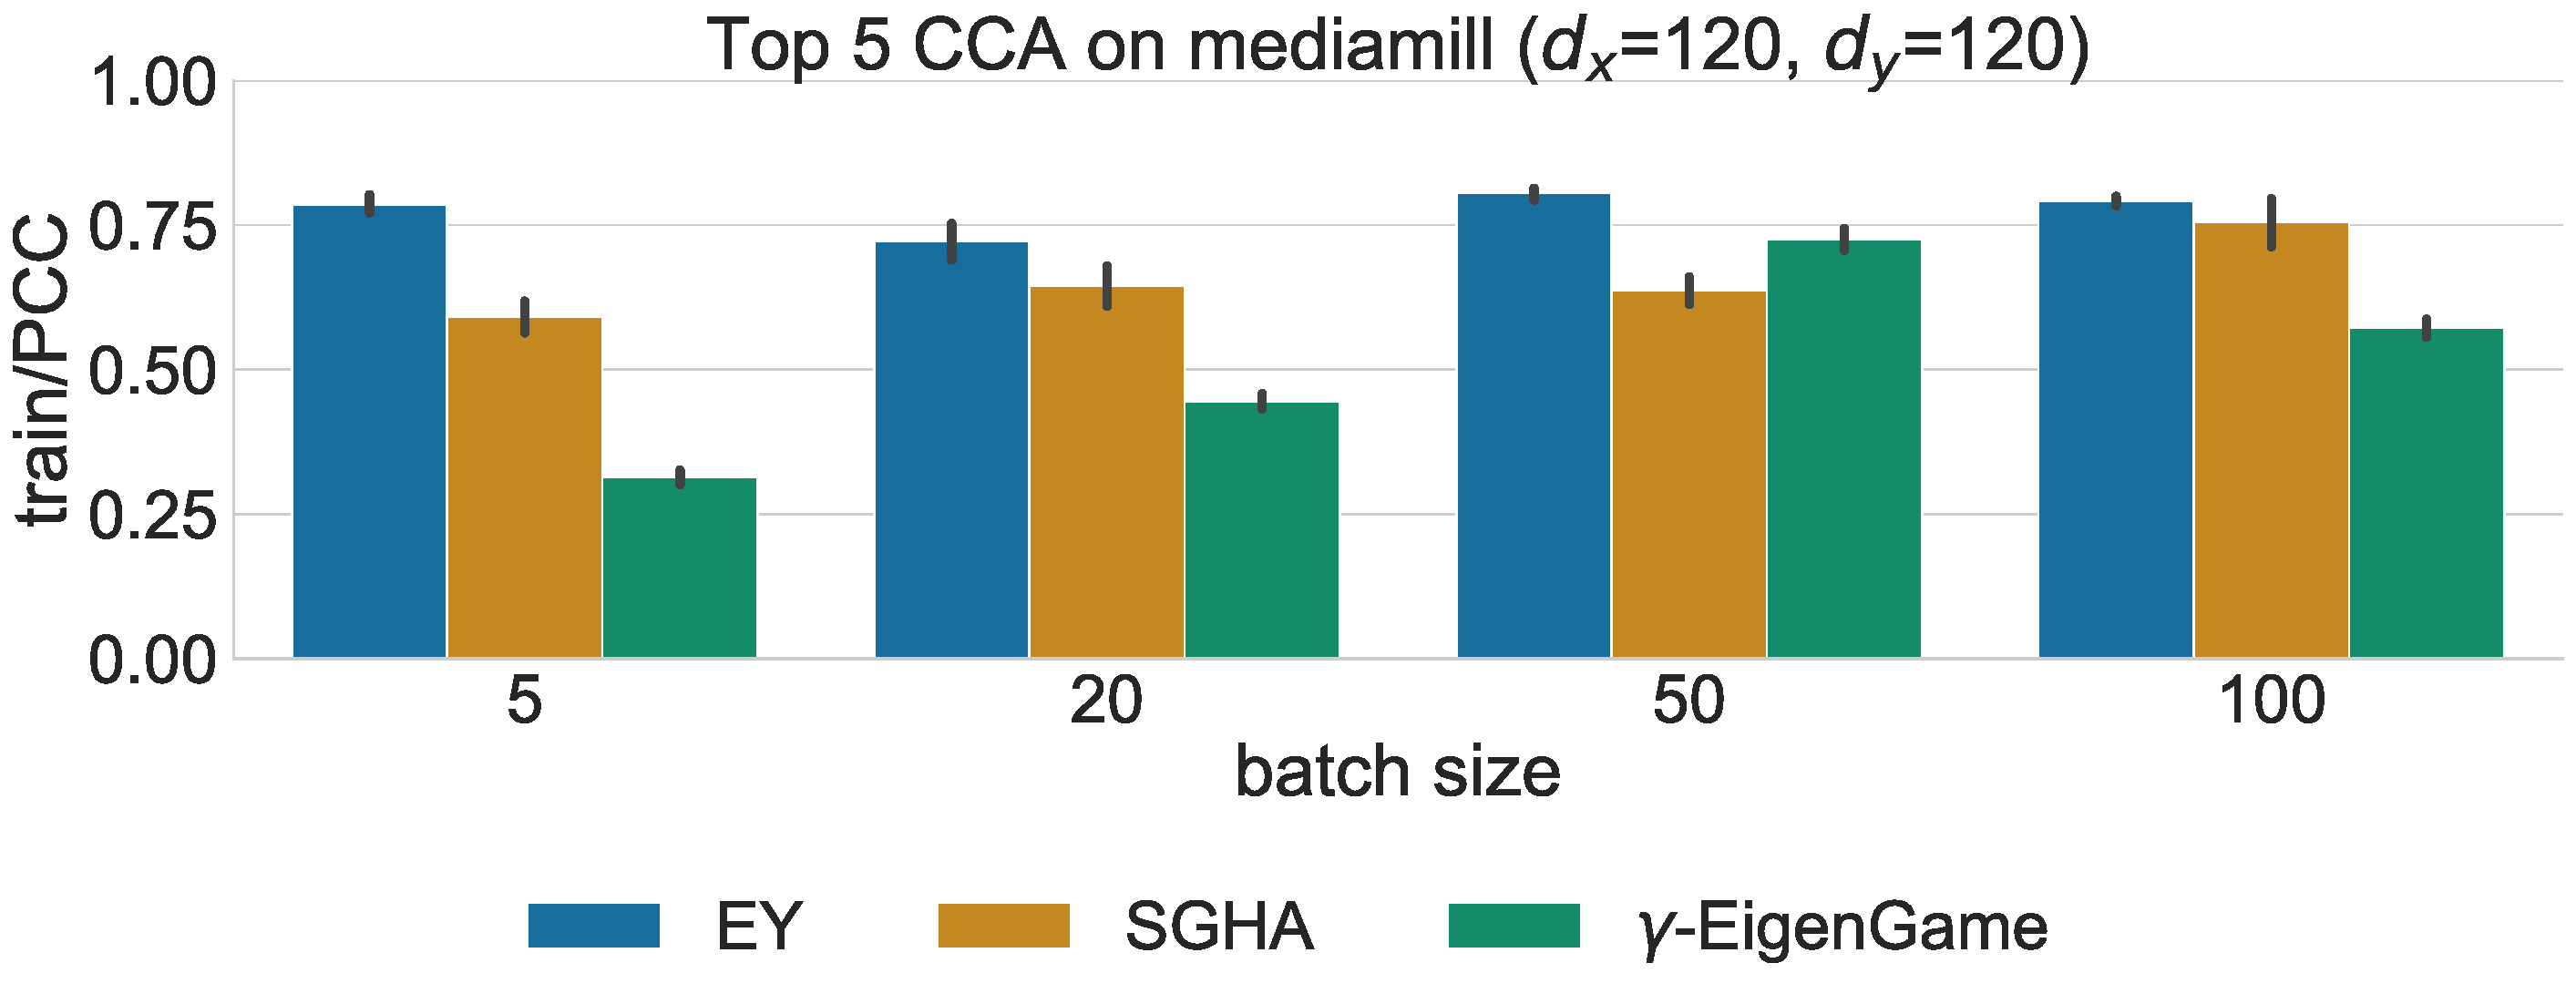
\includegraphics[width=\textwidth]{figures/CCA/mediamill_models_different_batch_sizes}
         \caption{}
         \label{fig:corr_mediamill}
     \end{subfigure}
     \hfill
     \begin{subfigure}[b]{0.49\textwidth}
         \centering
         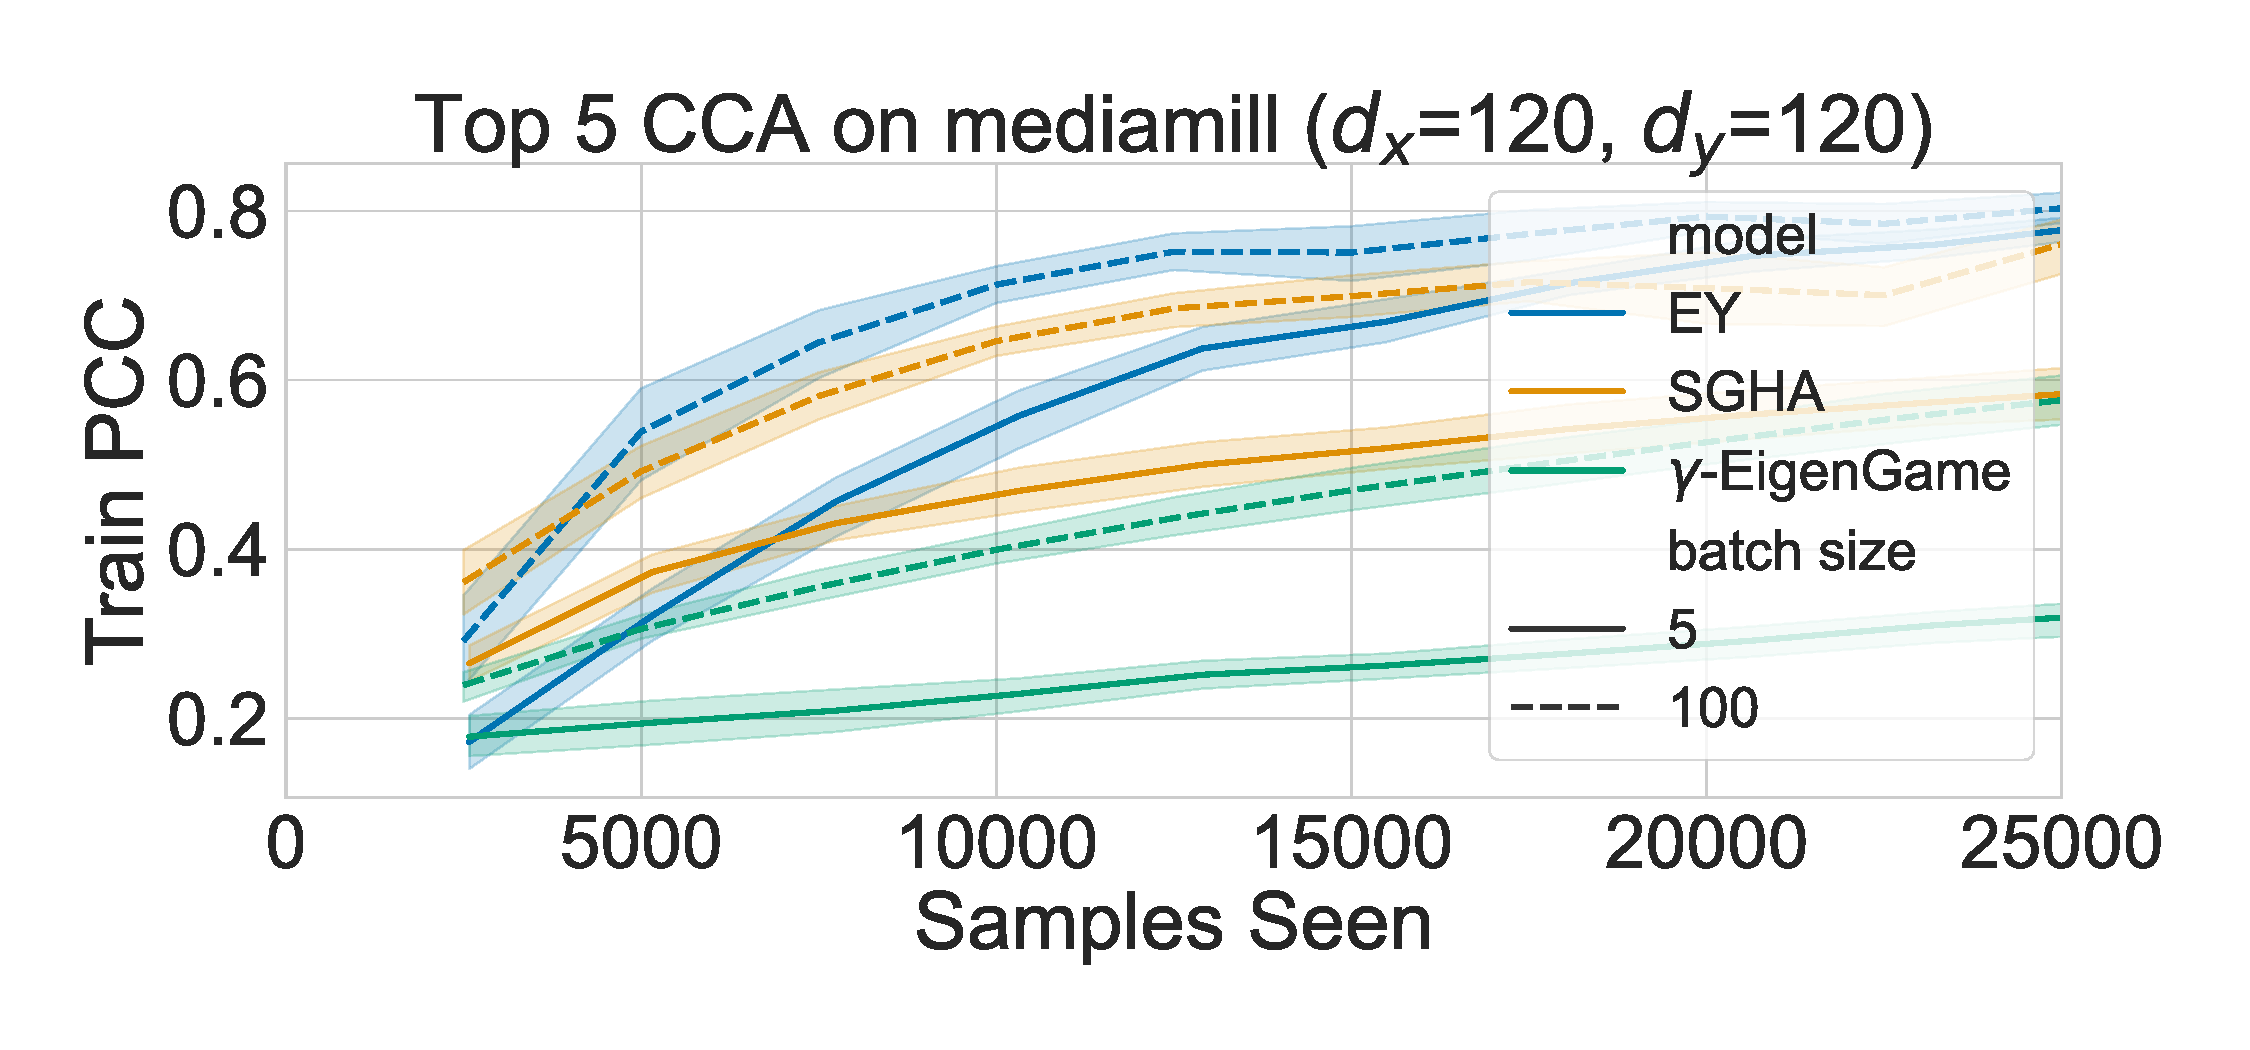
\includegraphics[width=\textwidth]{figures/CCA/mediamill_allbatchsizes_pcc}
         \caption{}
         \label{fig:lr_mediamill}
     \end{subfigure}
\caption{Stochastic CCA on MediaMill using the Proportion of Correlation Captured (PCC) metric: (a) Across varying mini-batch sizes, trained for a single epoch, and (b) Training progress over a single epoch for mini-batch sizes 5, 100.
%Both subfigures compare CCA-EY against prior methods ($\gamma$-EigenGame and SGHA).
Shaded regions signify \(\pm\) one standard deviation around the mean of 5 runs.}\label{fig:scca_mediamill}
\end{figure}



% Deep CCA Section
\subsection{Deep CCA}\label{sec:experiments-DCCA}
Second, we compare DCCA-EY against the DCCA methods described in \cref{sec:related-work}. The experimental setup is identical to that of \cite{wang2015stochastic}.
We learn $K=50$ dimensional representations, using mini-batch sizes ranging from 20 to 100 and train for 50 epochs.
Because there is no longer a ground truth we have to use Total Correlation Captured (TCC), given by \( \text{TCC} = \sum_{i=k}^K \rho_k \) where $\rho_k$ are now the empirical correlations between the representations on a validation set.

% In this section, we delve into the performance of DCCA-EY against other DCCA methods. The experimental setup is borrowed from \cite{wang2015stochastic}, utilizing the splitMNIST dataset. We use mini-batch sizes ranging from 20 to 100 and train the models for 50 epochs. Our metric here is the Total Correlation Captured (TCC), given by \( \text{TCC} = \sum_{i=1}^k \rho_i \).

\textbf{Observations:}
Figure \ref{fig: mnist} compares the methods on the splitMNIST dataset.
DCCA-STOL captures significantly less correlation than the other methods, and breaks down when the mini-batch size is less than the dimension $K=50$ due to low rank empirical covariances.
DCCA-NOI performs similarly to DCCA-EY but requires careful tuning of an additional hyperparameter, and shows significantly slower speed to convergence (Figure \ref{fig:lr_mnist}).

\textbf{Further experiments:} we conduct analogous experiments on the XRMB dataset in supplementary material \ref{app:xrmb_results} and observe identical behaviour.

\begin{figure}
     \centering
     \begin{subfigure}[b]{0.49\textwidth}
         \centering
         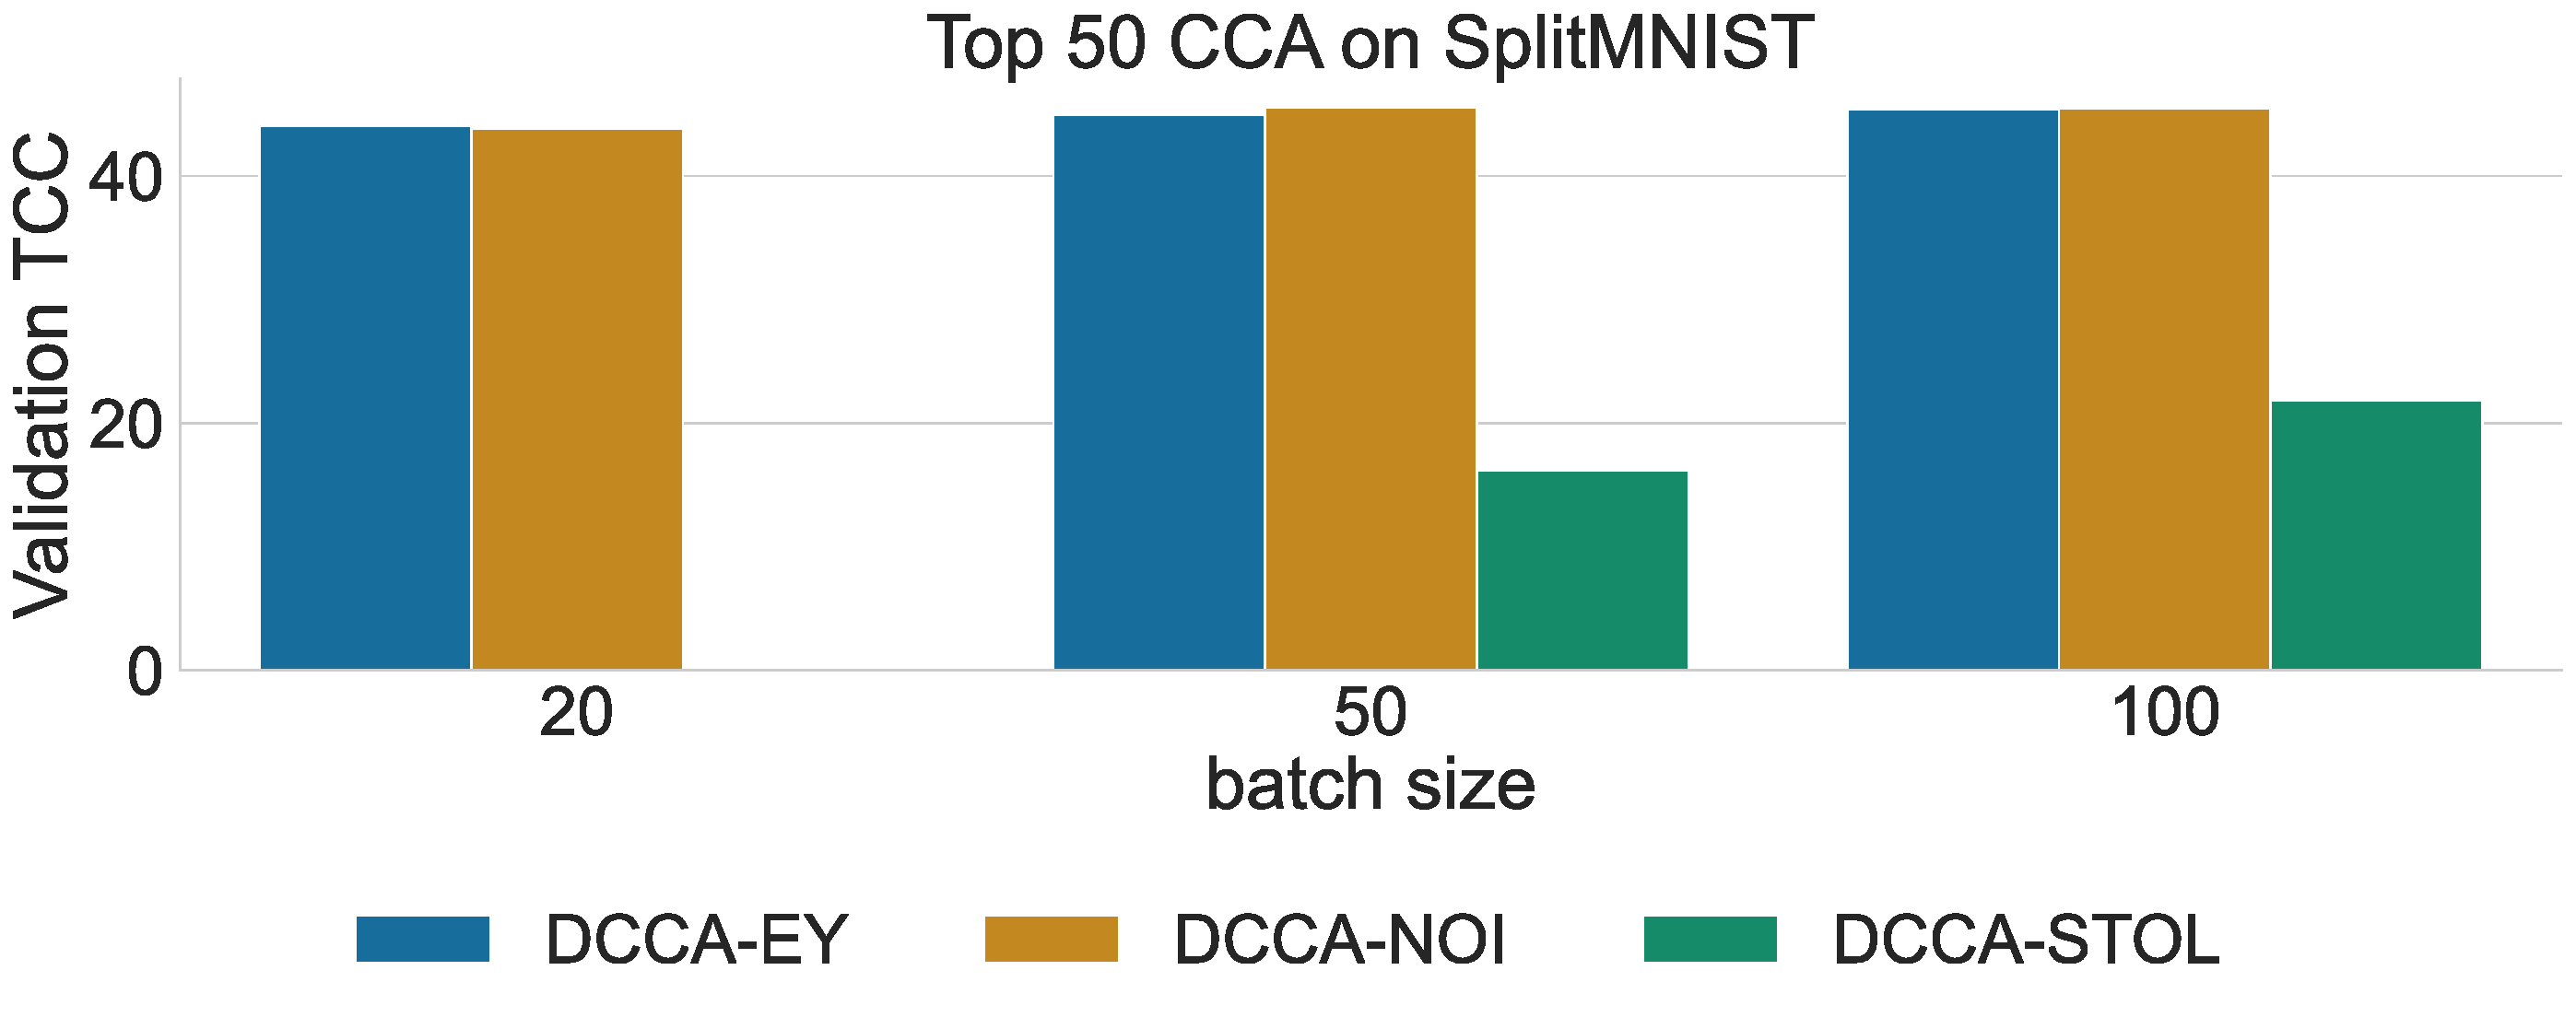
\includegraphics[width=\textwidth]{figures/DCCA/SplitMNIST_models_different_batch_sizes}
         \caption{}
         \label{fig:corr_mnist}
     \end{subfigure}
     \hfill
     \begin{subfigure}[b]{0.49\textwidth}
         \centering
         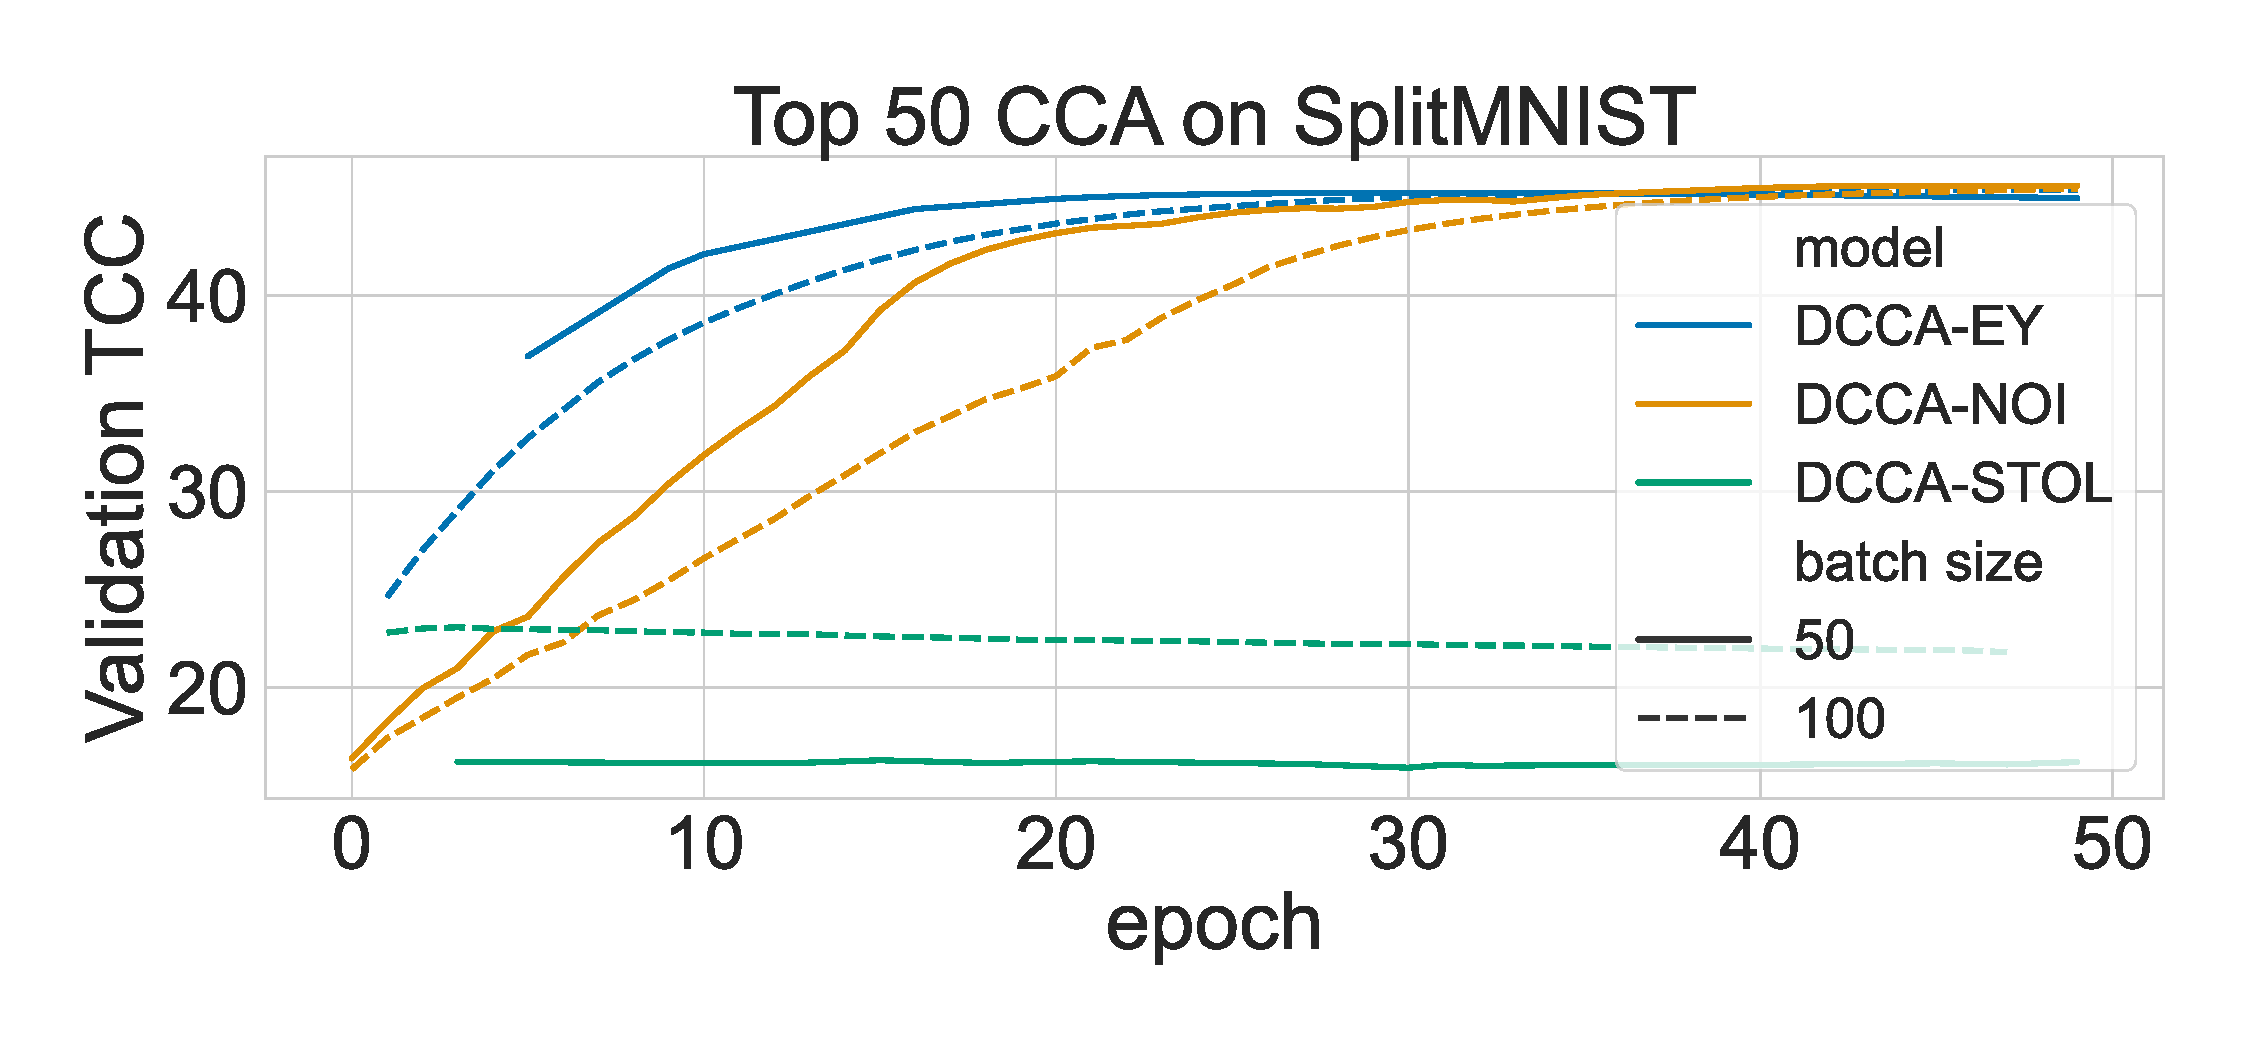
\includegraphics[width=\textwidth]{figures/DCCA/SplitMNIST_allbatchsizes_pcc}
         \caption{}
         \label{fig:lr_mnist}
     \end{subfigure}
\caption{Deep CCA on SplitMNIST using the Validation TCC metric: (a) after training each model for 50 epochs with varying batch sizes; (b) learning progress over 50 epochs.}
     \label{fig: mnist}
\end{figure}

\subsection{Deep Multiview CCA: Robustness Across Different Batch Sizes}
Third, we compare DCCA-EY to the existing DMCCA and DGCCA methods on the mfeat dataset; this contains 2,000 handwritten numeral patterns across six distinct feature sets, including Fourier coefficients, profile correlations, Karhunen-Love coefficients, pixel averages in \(2 \times 3\) windows, Zernike moments, and morphological features. We again learn $K=50$ dimensional representations, but now train for 100 epochs.
We use a multiview extension of the TCC metric, which averages correlation across views; we call this Total Multiview Correlation Captured (TMCC), defined as \(
\text{TMCC} = \sum_{k=1}^{K} \frac{1}{I(I-1)} \sum_{i,j \leq I, i\neq j} \text{corr}(Z_k^{(i)}, Z_k^{(j)}),
\) %where \(Z_k^{(i)}\) is the \(k\)-th dimension of the \(i\)-th view's representation,
using the notation of \cref{sec:background-unified}.

% In this subsection, we extend our analysis to multiview learning scenarios using the mfeat dataset. This dataset contains 2,000 handwritten numeral patterns across six distinct feature sets, including Fourier coefficients, profile correlations, Karhunen-Love coefficients, pixel averages in \(2 \times 3\) windows, Zernike moments, and morphological features. The architecture and training regimen adhere to those in our prior DCCA experiments, specifically comprizing 20 epochs with an output dimensionality of 50. We utilize the Total Multiview Correlation Captured (TMCC) as our evaluation metric, mathematically defined as \(
% \text{TMCC} = \sum_{d=1}^{50} \frac{1}{k(k-1)} \sum_{i=1}^k \sum_{j \neq i} \text{corr}(Z_i^{(d)}, Z_j^{(d)}),
% \) where \(Z_i^{(d)}\) is the \(d\)-th dimension of the \(i\)-th view's representation.

\textbf{Observations:}
Figure~\ref{fig:dmcca_corr} shows that DCCA-EY consistently outperforms both DGCCA and DMCCA across various mini-batch sizes in capturing validation TMCC.
Just like DCCA-NOI, DMCCA breaks down when the batch size is smaller than $K$. This is due to singular empirical covariances; DGCCA does not break down, but does significantly underperform with smaller batch sizes.
This limits their practical applicability to large-scale data.
Figure~\ref{fig:dmcca_lr} shows learning curves for batch sizes 50 and 100.
DMCCA and DGCCA both quickly learn significant correlations but then plateau out; our method consistently improves, and significantly outperforms them by the end of training.

% Our DCCA-EY model consistently outperforms the DGCCA and DMCCA methods across various mini-batch sizes in capturing validation TMCC, as illustrated in Figure~\ref{fig:dmcca_corr}. This establishes the robustness and efficiency of our approach in multiview settings. Additionally, we note that while some competing models may converge swiftly with larger batch sizes, they fail to do so at smaller ones, limiting their practical applicability (see Figure~\ref{fig:dmcca_lr} for learning curve details).

\begin{figure}
     \centering
     \begin{subfigure}[b]{0.49\textwidth}
         \centering
         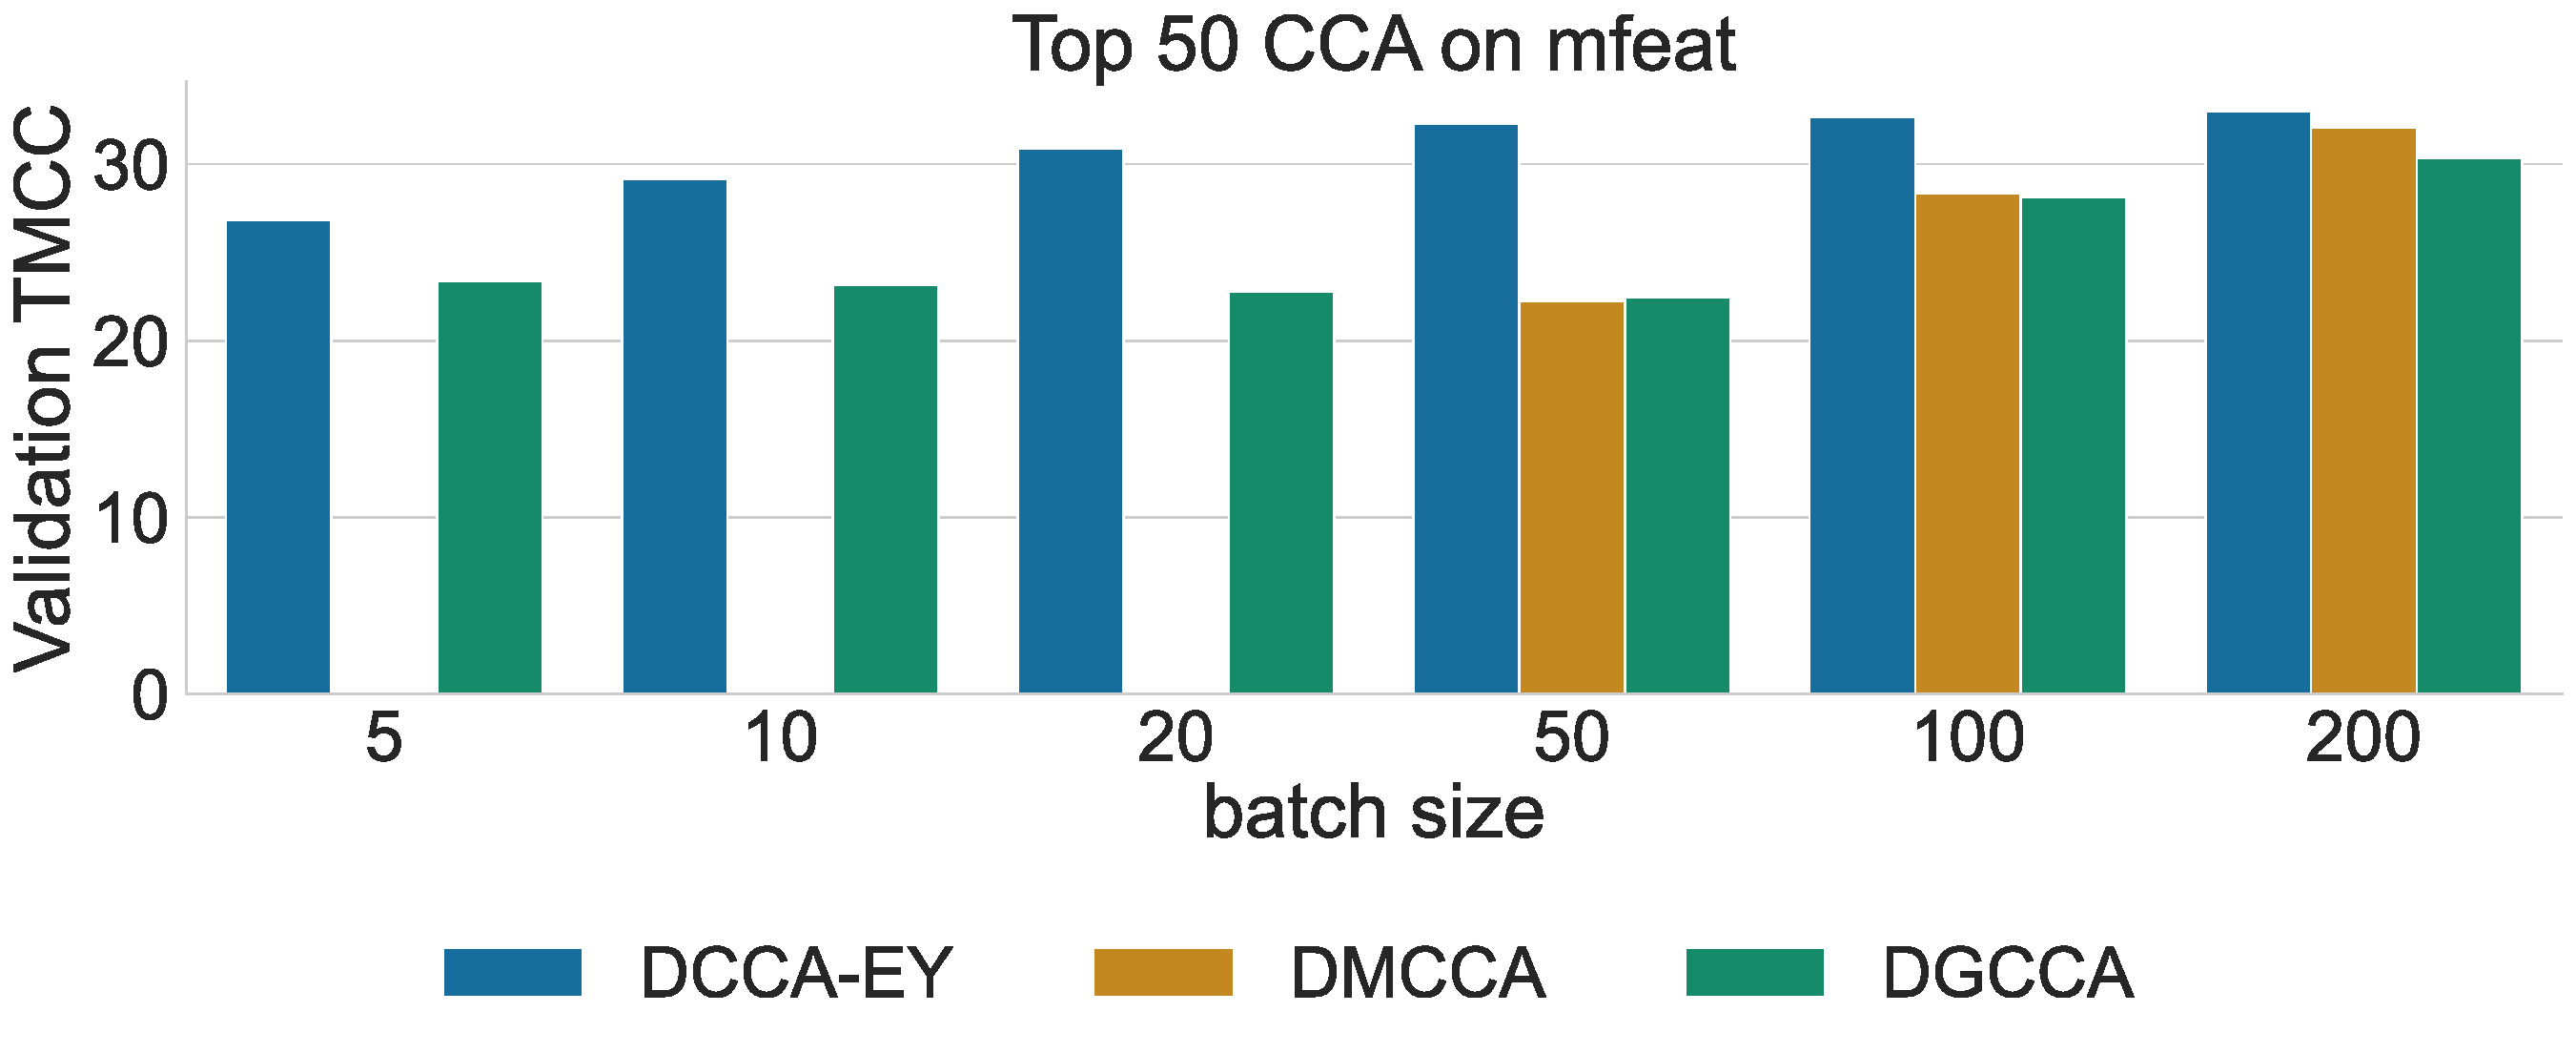
\includegraphics[width=\textwidth]{figures/DMCCA/mfeat_models_different_batch_sizes}
         \caption{}\label{fig:dmcca_corr}
     \end{subfigure}
     \hfill
     \begin{subfigure}[b]{0.49\textwidth}
         \centering
         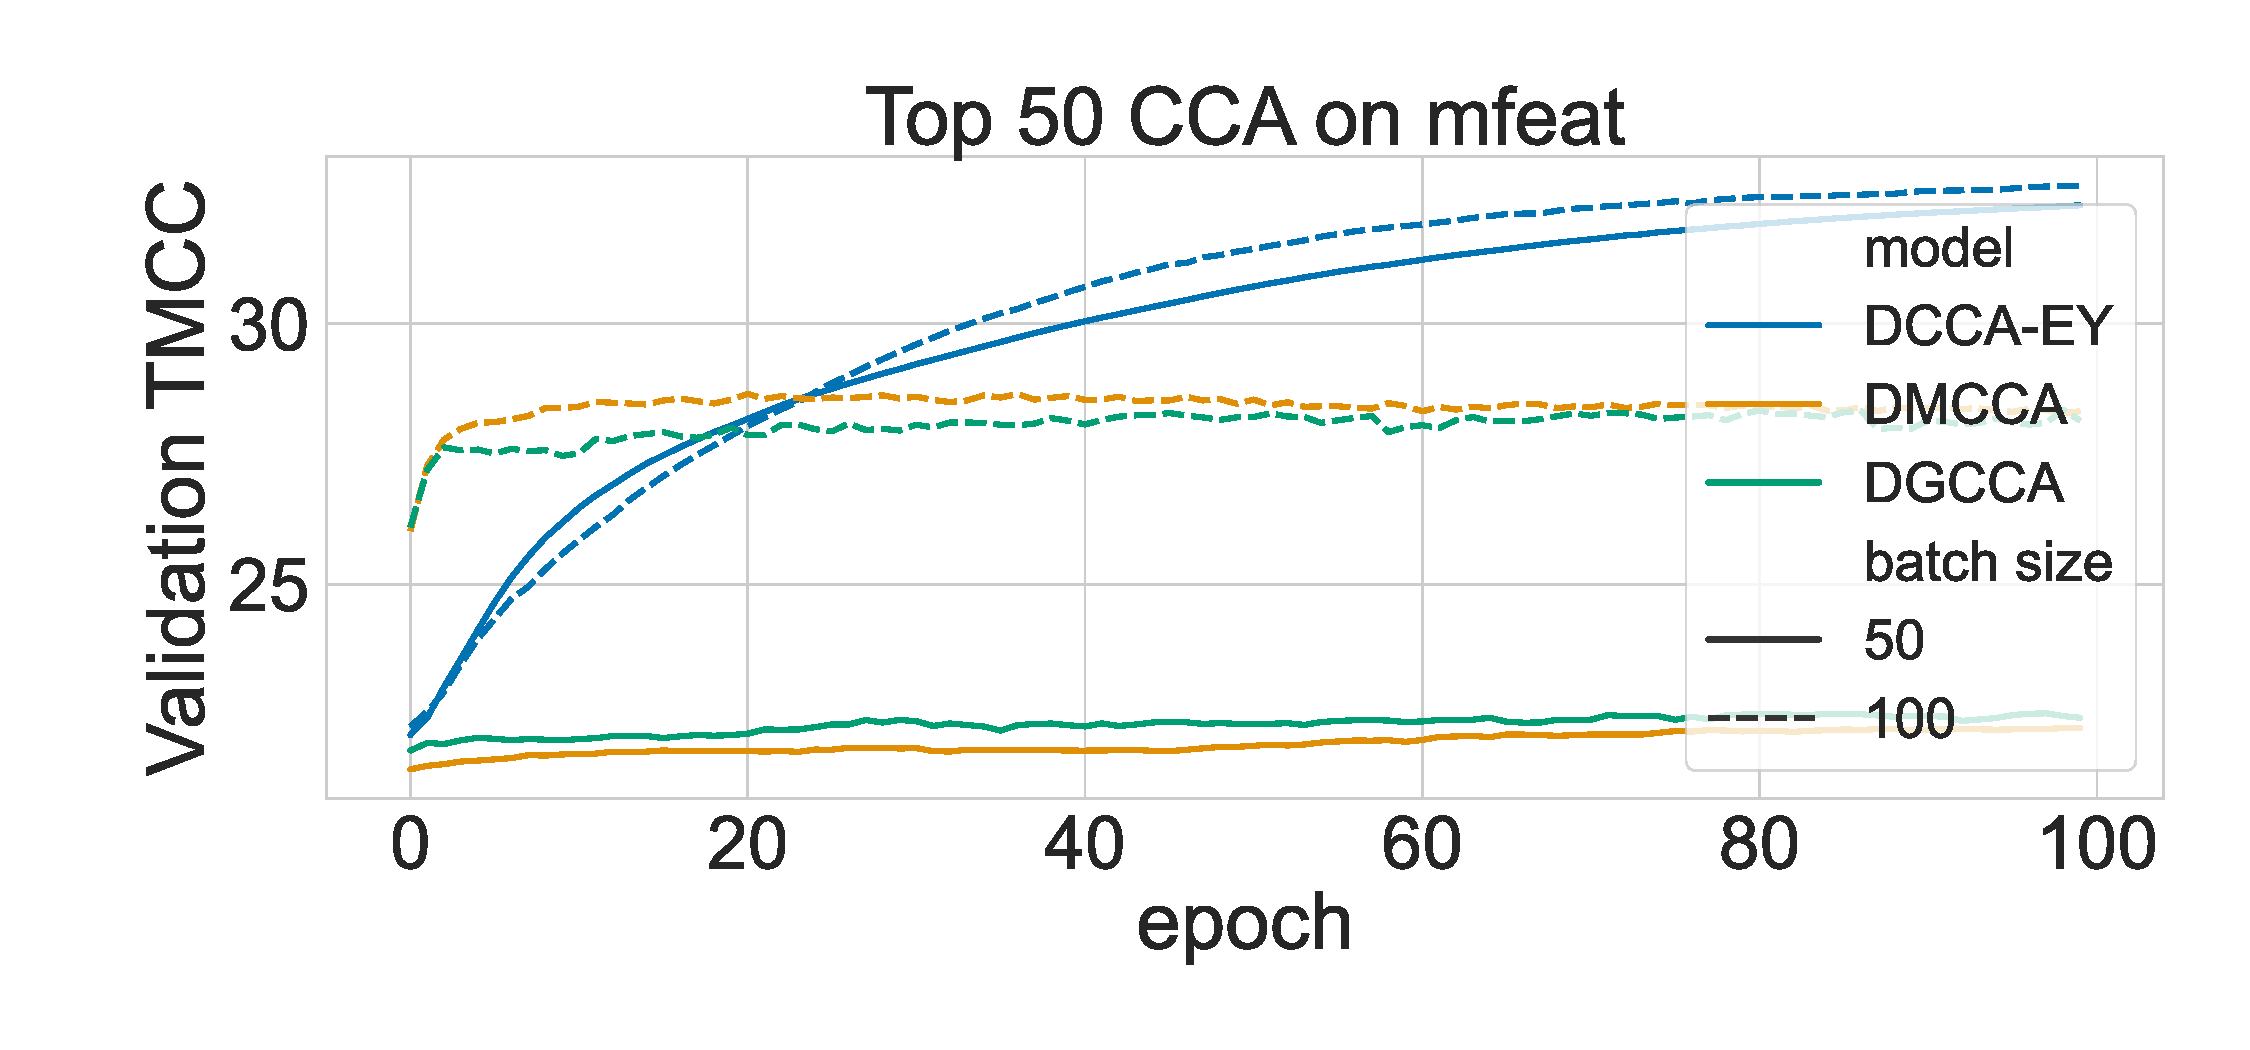
\includegraphics[width=\textwidth]{figures/DMCCA/mfeat_allbatchsizes_pcc}
         \caption{}\label{fig:dmcca_lr}
     \end{subfigure}
     \caption{Deep Multi-view CCA on mfeat using the Validation TMCC metric: (a) after training each model for 100 epochs with varying batch sizes; (b) learning progress over 100 epochs.}
     \label{fig:dmcca}
\end{figure}


\subsection{Stochastic PLS UK Biobank}
Next, we demonstrate the scalability of our methods to extremely high-dimensional data by applying stochastic PLS to imaging genetics data from the UK Biobank \citep{sudlow2015uk}.
PLS is typically used for imaging-genetics studies owing to the extremely high dimensionality of genetics data requiring lots of regularisation.
PLS can reveal novel phenotypes of interest and uncover genetic mechanisms of disease and brain morphometry.
Previous imaging genetics analyses using full-batch PLS were limited to much smaller datasets \citep{Lorenzi2018,Taquet2021,Lefloch2012}.
The only other analysis on the UK Biobank at comparable scale partitions the data into clusters and bootstrapping local PLS solutions on these clusters \citep{lorenzi2017secure, altmann2023tackling}.
We ran PLS-EY with mini-batch size 500 on brain imaging (82 regional volumes) and genetics (582,565 variants) data for 33,333 subjects. See supplement (Section \ref{sec:ukbb_preprocessing}) for data pre-processing details.
To our knowledge, this is the largest-scale PLS analysis of biomedical data to-date.

\textbf{Observations:} We see strong validation correlation between all 10 corresponding pairs of vectors in the PLS subspace and weak cross correlation, indicating that our model learnt a coherent and orthogonal subspace of covariation (Figure \ref{fig:UKBB_corr}), a remarkable feat for such high-dimensional data. We found that the PLS brain subspace was associated with genetic risk measures for several disorders (Figure \ref{fig:genetic_risk}), suggesting that the PLS subspace encodes relevant information for genetic disease risk, a significant finding for biomedical research.

\begin{figure}
\centering
     \begin{subfigure}[b]{0.27\textwidth}
         \centering
          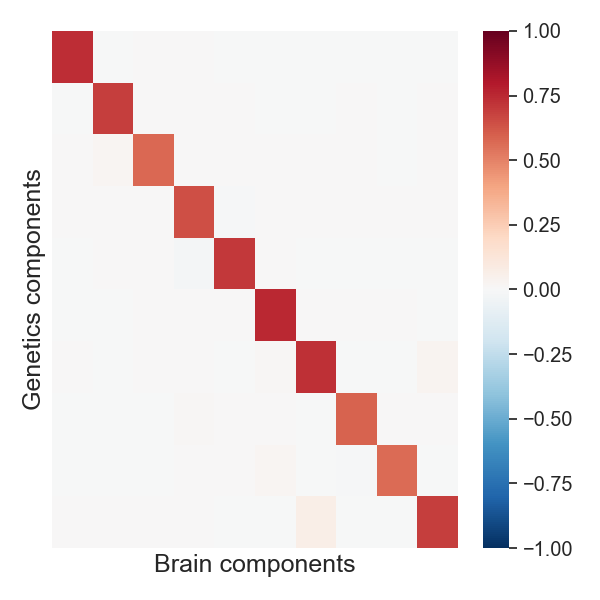
\includegraphics[width=\textwidth,trim={0.8cm 0cm 0.3cm 0cm}]{figures/UKBB/cross_corr.png}
          \caption{}
          \label{fig:UKBB_corr}
     \end{subfigure}
     \begin{subfigure}[b]{0.72\textwidth}
         \centering
          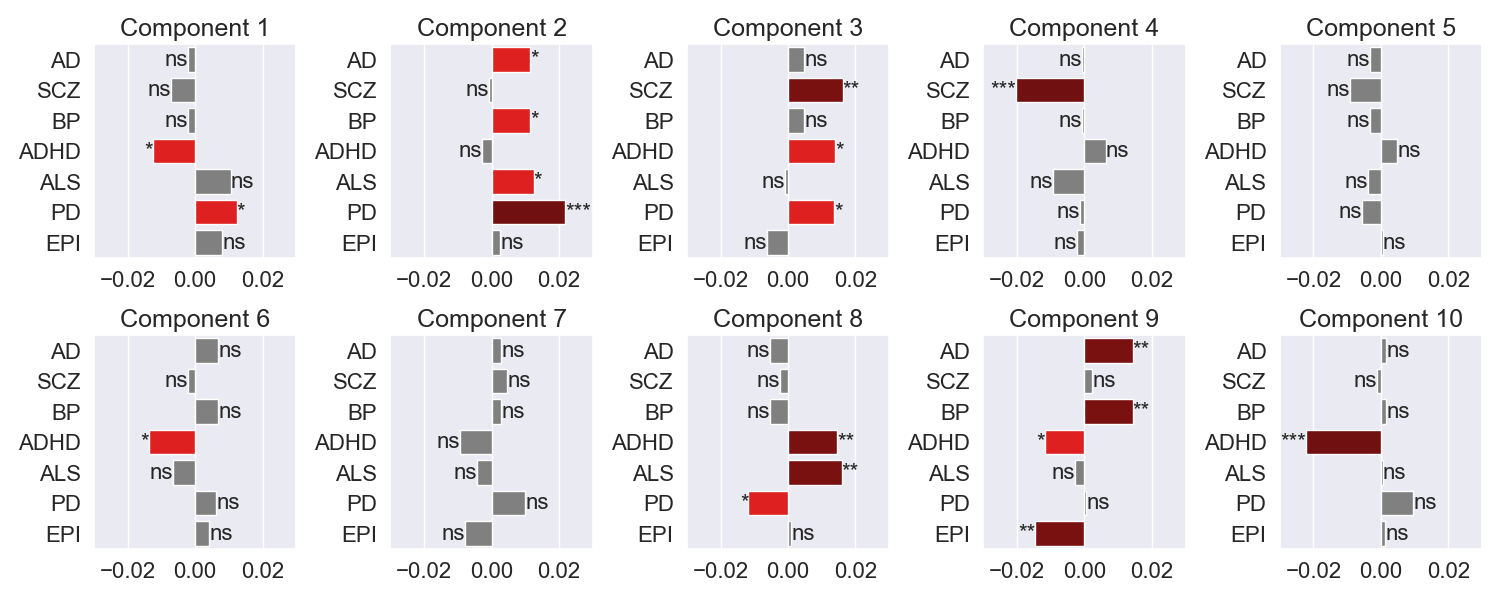
\includegraphics[width=\textwidth,trim={0.5cm 0cm 0.7cm 0cm}]{figures/UKBB/prs_correlations.png}
          \caption{}
          \label{fig:genetic_risk}
     \end{subfigure}
\caption{(a) Correlations between PLS components for UK Biobank. (b) Correlations between PLS brain components and genetic risk scores. AD=Alzheimer's disease, SCZ=Schizophrenia, BP=Bipolar, ADHD=Attention deficit hyperactivity disorder, ALS=Amyotrophic lateral sclerosis, PD=Parkinson's disease, EPI=Epilepsy. $\text{ns}: 0.05< p <= 1, \ast: 0.01< p <=0.05, \ast\ast: 0.001< p <= 0.01, \ast\ast\ast: 0.0001< p <= 0.001$.}
\end{figure}

\subsection{Self-Supervised Learning with SSL-EY}
Finally, we benchmark our self-supervised learning algorithm, SSL-EY, with Barlow Twins and VICReg on CIFAR-10 and CIFAR-100. Each dataset contains 60,000 labelled images, but these are over 10 classes for CIFAR-10 and 100 classes for CIFAR-100.

We follow a standard experimental design \citep{tong2023emp}. Indeed, we use the sololearn library \citep{da2022solo}, which offers optimized setups particularly tailored for VICReg and Barlow Twins. All methods utilize a ResNet-18 encoder coupled with a bi-layer projector network. Training spans 1,000 epochs with batches of 256 images. For SSL-EY, we use the hyperparameters optimized for Barlow Twins, aiming not to outperform but to showcase the robustness of our method.
We predict labels via a linear probe on the learnt representations and evaluate performance with Top-1 and Top-5 accuracies on the validation set. For more details, refer to the supplementary material \ref{supp:experimental details}.

\textbf{Observations:} Table \ref{tab:selfsup} shows that SSL-EY is competitive with Barlow Twins and VICReg. This is remarkable because we used out-of-the-box hyperparameters for SSL-EY but used hyperparameters for Barlow Twins and VICReg that had been heavily optimized in previous studies.

\textbf{Further experiments} included in \cref{supp:SSL} show that the learning curves for all three methods are comparable, and that our method is much more stable when reducing the dimension of the learnt representations.

\begin{table}
    \centering
    \begin{tabular}{lcccc}
        \hline
        Method & CIFAR-10 Top-1 & CIFAR-10 Top-5 & CIFAR-100 Top-1 & CIFAR-100 Top-5 \\
        \hline
        Barlow Twins & \textbf{92.1} & 99.73 & \textbf{71.38} & \textbf{92.32} \\
        VICReg & 91.68 & 99.66 & 68.56 & 90.76 \\
        \textbf{SSL-EY} & 91.43 & \textbf{99.75} & 67.52 & 90.17 \\
        \hline
    \end{tabular}
    \caption{Performance comparison of SSL methods on CIFAR-10 and CIFAR-100.}
    \label{tab:selfsup}
\end{table}


\section{Conclusion}

In this paper, we introduced a class of efficient, scalable algorithms for Canonical Correlation Analysis and Self-Supervised Learning, rooted in a novel unconstrained loss function. These algorithms are computationally lightweight, making them uniquely suited for large-scale problems where traditional methods struggle.

We have two distinct avenues for future research. Firstly, we aim to incorporate regularization techniques to improve both generalizability and interpretability, building upon existing sparse methods in CCA \citep{witten2009extensions}. We also intend to investigate the utility of correlation as a metric for measuring the quality of learnt representations. This holds the potential to replace traditional validation methods like classification accuracy, especially in situations where validation labels are not available.

In summary, this paper sets a new benchmark for addressing large-scale CCA problems and opens new avenues in self-supervised learning, paving the way for more accessible and efficient solutions in various applications.